%%%%%%%%%%%%%%%%%%%%%%%%%%%%%%%%%%%%%%%%%%%%%%%%%%%%%%%%%%%%%%%%%%%%%%%%%%%%%
\chapter{Hauptteil}
\label{chap:intro}
%%%%%%%%%%%%%%%%%%%%%%%%%%%%%%%%%%%%%%%%%%%%%%%%%%%%%%%%%%%%%%%%%%%%%%%%%%%%%
\chapterstart

\section{Theoretischer Hintergrund:}

In diesem Kapitel soll eine Basis für die Grundlegenden Technologien, Standards und Begriffe geschaffen werden, welche im Zuge der wissenschaftlichen Arbeit verglichen bzw. verwendet wurden.

Die Arbeit Untersucht die Kommunikation zwischen Frontend zu Backend Komponenten, im industriellen als auch wissenschafltichem Kontext sind diese Begriffe wie folgt definiert:

\chapquote{Das Frontend ist das, was Ihre Benutzer sehen, und enthält visuelle Elemente wie Schaltflächen, Kontrollkästchen, Grafiken und Textnachrichten. Es ermöglicht den Benutzern, mit Ihrer Anwendung zu interagieren. Das Backend sind die Daten und die Infrastruktur, die dafür sorgen, dass Ihre Anwendung funktioniert. Es speichert und verarbeitet Anwendungsdaten für Ihre Benutzer.}
{\cite{awsfrontendbackend}}

Wie aus dieser Definition ersichtlich beinhaltet das Front-End den benutzerspezifischen Teil und das backend den Datenverarbeitungsteil. Im Zuge der Bachelorarbeit werden anschlieden für die Front End Komponente ebenso das Wort „Client“ und für die Backend Komponente das wort „Server“ verwendet.

\subsection{Serialisierungsformate}
Bei der Übertragung zwischen der Front-End und Back-End Komponente werden Daten ausgetauscht. Da es eine Vielzahl an Technologien gibt, mit denen die jeweiligen Komponenten realisiert werden können, wurden Standards definiert, damit diese sinnvoll und effizient verarbeitet werden können.

\subsubsection{JSON}
JSON steht für JavaScript Object Notation und ist ein weit verbreitetes, textbasiertes Datenformat, das vorallem wegen einfacher Lesbarkeit und breiter Unterstützung in vielen Programmiersprachen Verwendung findet. Das Format basiert auf einer Schlüssel-Wert Paar Struktur mit einfacher Syntax ( Klammern, Spalten, Doppelpunkte, Kommas ) und kann folgende Datentypen annehmen:

\begin{itemize}
	\item String (Zeichenkette)
	\item Number (Zahl)
	\item Boolean (true/false)
	\item Array (Liste)
	\item Object (Objekt mit weiteren Schl\"ussel-Wert-Paaren)
	\item null (leerer Wert)
\end{itemize}


JSON ist der Standard für REST und GraphQL Schnittstellen.


\subsubsection{Protocol Buffers}
Protocol Buffer sind ein von Google entwickeltes Serialisierungsformat. Es handelt sich hierbei um ein binäres Serialisierungsformat, das entwickelt wurde um möglichst effizient, mit hoher Performance und mit so wenig Overhead wie möglich (ohne Whitespaces oder Satzzeichen wie bei JSON) Daten zu übertragen und zu verarbeiten. Protocul Buffer sind Plattform unabhängig und mit den meisten gängigen Programmiersprachen kompatibel.

Ein zentraler Bestandteil Protocol Buffer sind dabei plattformunabhängigen .proto Files, die für die Erzeugung definiert werden müssen.

Mit den definierten .proto Files können anschließend mit einem Plattform Abhängigen Protobuf-Compiler-Tool ( z.B. protoc ) Datenobjekte der jeweiligen Programmiersprache generiert werden.


\newpage
\textbf{\underline{Aufbau der .proto Files}}
\newline
Hauptbestandteil der .proto Files sind messages und services.

\begin{verbatim}
	message Person {
		string name = 1;
		int32 id = 2;
		string email = 3;
	}
\end{verbatim}

Messages geben dabei die Struktur der zu übertragenden Nachricht und den jeweiligen Datentypen an und einer Nummer, die beschreibt an welcher Stelle sich das jeweilige Attribut befindet, an. Die Nummerierung der Felder ist wichtig für die Serialisierung.
In Protocol Buffers können unter anderem die gängigsten Datentypen wie int32, int64, float, double, bool sowie string und bytes verwendet werden.

\begin{verbatim}
	service PersonService {
		rpc GetPerson (PersonRequest) returns (Person);
	}
\end{verbatim}

Services geben an, welche Dienste vom Server bereit gestellt werden und welche Datentypen als Parameter bei Aufruf übermittelt und als Rückgabe zurückgegeben werden. Services müssen auf der Seite des zur Verfügung stellenden Dienstes ausimplementiert werden.

Das Protobuf Serialisierungsformat wurde vorallem für die inter-server Kommunikation ( innherhalb der Backend seitigen Kommunikation) entwickelt, im Zuge der Bachelorarbeit wird diese auf die Verwendung in der Frontend zu Backend Kommunikation untersucht.

\subsection{Übertragung binärer Daten (Blob)}:
Für das Übertragen von großen binären Objekten ( wie Bilder, Video, Audiodateien, Dokumente, .. ) wird eine große Menge an binären Daten ( Datentyp: byte) gesendet. Solche großen binären Dateien, die bei der Kommunikation zwischen Client und Server gesendet werden, werden in der Webentwicklung, und vorallem im Frontend wo diese Mediendaten verarbeitet werden sollen, oft als Blob ( Binary Large Object ) bezeichnet. 


\subsection{Transportprotokolle}
Die eigentlichen Daten, die in Form von Serialisierungsformaten zwischen Frontend und backend ausgetauscht werden, werden mithilfe von Transportprotokollen von dem Client and den Server, und umgekehrt, übermittelt. Das Hypertext Transfer Protocol (http) ist dabei für moderne Webanwendungen das zentrale und verbreitetste Transportprotokoll. Im Kontext der Bachelorarbeit, wird insbesondere auf zwei Versionen von http eingegangen:

\subsubsection{HTTP/1.1}

http/1 Ist der momentan am weitesten verbreitetste Protokoll für die Kommunikation zwischen Frontend und Backend anwendungen. Es wird von allen Webbrowsern ohne einschränkungen unterstützt und bildet die Grundlage für die API Technologien REST und GraphQL. Das Protokoll funktioniert mittels eines request-responds Prinzips und überträgt die Daten über eine textbasierte Verbindung mittels eines TCP Transportprotokolls. 

\begin{figure}[htbp]
	\centering
	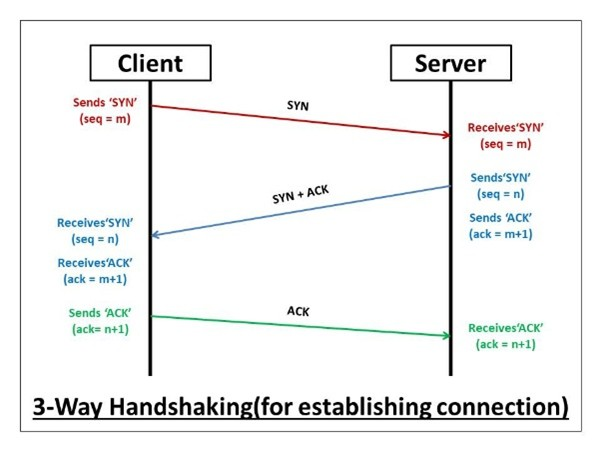
\includegraphics[width=0.7\textwidth]{images/http1_theory.jpg}
	\caption{3-Way Handshake (for establishing TCP connection)}
	\label{fig:threewayhandshake}
\end{figure}

Der Verbindungsaufbau erfolgt dabei mittels eines Transmission Control Protocol  (TCP) – Handshakes, welcher für eine zuverlässige Verbindung zwischen zwei Systemen verwenden wird. Dabei werden in drei Schritten Steuerpakete ausgetauscht:

1. Zuerst sendet der Client ein SYN (Synchronize( – Paket an den Server

2. Der Server antwortet mit einem SYN – ACK ( Acknowledge) Paket

3. Der Cient antwortet mit einem ACK

Ernst nach diesen Schritten, gilt die Verbindung als aufgebaut und die Daten werden übertragen.

Vorallem wegen der sequentielle Abarbeitung  und die Notwendigkeit von mehreren Verbindungen bei parallelen Requests führt häufig zu Performance Einschränkungen, welche vorallem bei dantenintensiven Anwendungen zu Problemen führen kann. 


\subsubsection{HTTP/2}
Aufgrund der ber http/1 genannten Performance Problemen wurde eine neue Version namens http/2 Enwickelt, weche viele Schwächen von http/1.1, insbesondere beszogen auf Latenz und Effizienz, ausgleicht.
Das Hauptmerkmal von http/2 ist Multiplexing, hierbei ist es möglich mehrere parallele Anfragen und Antworten über nur eine einzige TCP-Verbindung durchzuführen.
Weitere Verbesserungen beinhalten zum Beispiel die Komprimierung von Header-Informationen oder das Server Push-Verfahren, das eine proaktive Übertragung vom Server an den Client erlaubt.
Aufgrund der oben genannten Verbesserungen wird http/2 besonders in modernen Anwendungen in denen eine schnelle und effiziente Datenübertragung wichtig ist, wie biespielsweise bei gRPC, Echtzeitkommunikation oder Microservices verwendet.
Webbrowser unterstützen nur eine eingeschränkte Nutzung von http/2 deshalb können bei der Kommunikation zwischen Webbrowsern und Serveranwendungen nicht alle Vorteile ausgenutzt werden. Zwar unterstützen aktuelle Webbrowser mittlerweile http/2, jedoch ist bei der verwendung eine verschlüsselte Übertragung verpflichtend, und wichtige Features wie echted bidirektionales Streaming (gleichzeitiges Senden und Empfangen von Daten durch Client und Server) oder http/2 Trailers (das Übermitteln zusätzlicher Metadaten am Ende einer Übertragung, z.B. zur Fehlerbehandlung, welche bei gRPC zum einsatz kommen, werden in Webbrowsern nicht bzw. nur teilweise unterstützt. Dadurch können bei der Kommunikation zwischen Frontend (Webbrowser) und Backend nicht alle Potenziale von HTTP/2 ausgeschöpft werden 


\subsection{API-Technologien}
Eine API ist eine Schnittstelle eines Softwaremoduls, welche es ermöglicht, dass das jeweilige Softwaresystem mit einem anderem System kommunizieren kann.
Eine Web API sind APIs die von Web-Servern zur Verfügung gestellt werden. Bei webservern findet die Kommunikation mit einem der http bzw. https Protokollen statt. Da sich die Forschungsfragen und der Prototyp gezielt auf die Kommunikation zwischen einem Web Frontend und einem Webserver beziehen, bezieht sich der Begriff API im folgenden immer auf Web APIs.

API Technologien wie REST, GraphQL oder gRPC legen Standards fest ( Konventionen, Art der Serialisierungsobjekte, Art des Transportprotokolls) die neben der technischen Kompatibilität für die Kommunikation auch Entwicklern hilft, sich effizient in API-Systemen zurecht zu finden.


\subsubsection{Representational State Transfer (REST)}

Der REST-Architekturstuk wure im Jahr 1994 von Roy Fielding im Rahmen seiner Dissertation entwickelt, mit dem Ziel eine bis dato einfache Alternative für die Kommunikation zwischen zwei Systemen zu schaffen. 

\textbf{\underline{Infrastruktur:}}
Eine API-Schnittstellt ist nach Definition nur dann im REST Stil umgesetzt, falls folgende 5 Eigenschaften erfüllt werden:


\begin{itemize}
	\item \textbf{Client-Server:}
	Das System muss sich in einer Server-Client Architektur umgesetzt werden. Besteht aus einem Server, der einen Dienst oder Daten bereitstellt und einem Client, welcher diese Dienste nutzen kann. Server und Client kommunizieren mittels Nachrichten, indem mittel eines Request-Respond Prinzips der Client eine Anfrage (Request) schickt und der Server eine Antwort (Respond)
	zurückliefert.
	
	\item \textbf{Zustandslosigkeit:} 
	In jeder Nachricht, die zwischen Server-Client verschickt werden müssen alle Informationen enthalten sein, damit der jeweilige Kommunikationspartner die Nachricht verarbeiten kann. Es ist nicht erlaubt Zustandsinformationen zwischen zwei Nachrichten zu speichern.
	\item \textbf{Caching:}
	HTTP Caching soll benutzt werden, hierbei werden Daten in einem Cache gespeichert und bei nochmaligem abfragen vom Cache abgefragt, um unnötige Serveranfragen und Datenübertragungen zu vermeiden.
	\item \textbf{Einheitliche Schnittstelle:}
	Eine einheitliche Schnittstelle ist wie folgt definiert:
	
	\begin{enumerate}
		\item \textbf{Addressierbarkeit von Ressourcen:}
		Jede Ressource im System ist eindeutig über eine URI adressierbar.
		\item \textbf{Repräsentationen zur Veränderung von Ressourcen:}
		Ressourcen können durch verschiedene Formate (wie JSON oder XML) repräsentiert und über Standard-HTTP-Methoden verändert werden.
		
		\item \textbf{Selbsbeschreibende Nachrichten:}
		Jede Nachricht enthält alle notwendigen Informationen, damit der Empfänger sie interpretieren und verarbeiten kann.
		
		\item \textbf{„Hypermedia as the Engine of Application State“ (HATEOAS):} 
		Bei HATEOAS stellt der Server dem Client Links zur Verfügung, mittels dem der Client auf weitere Ressourcen zugreifen kann.
	\end{enumerate}
	
	\item \textbf{Mehrschichtige Systeme:}
	Systeme sollen mehrschichtig aufgebaut sein, die Kommunikationsparner müssen aber jeweils immer nur die oberste Schicht kennen.
	
	\item \textbf{Code on Demand (optional):}
	Im Bedarfsfall kann der Server dem Client Code zur Verfügung stellen. Diese Eigenschaft ist für einen REST Architekturstil jedoch nur optional.
\end{itemize}

Viele Web Dienste, erfüllen bereits viele dieser Eigenschaften wodurch sich REST zu einem beliebten Standard entwickelt hat.

\textbf{\underline{Kommunikation zwischen Client – Server:}}
Die Kommunikation zwischen dem findet bei REST fast ausschließlich über http/HTTPs statt, wobei laut Definition kein spezifisches Transportprotokoll vorgeschrieben wird. Im Zuge der Arbeit und der weiten Verbreitung wird im Zuge der Arbeit ausschließlich http verwendet.

HTTP stellt für den Zugriff auf Ressourcen eine Reihe an Methoden zur Verfügung. Die wichtigsen http Methoden sind : \newline

\begin{tabularx}{\textwidth}{|l|X|}
	\hline
	\textbf{HTTP Methode} & \textbf{Beschreibung} \\
	\hline
	GET & GET fordert eine Ressource vom Server an. Der Zustand des Dienstes bzw.\ der Ressource wird dabei nicht verändert. \\
	\hline
	POST & Fügt in den meisten Fällen eine neue Ressource ein. Kann aber auch verwendet werden, um Methoden zu realisieren, die durch keine andere HTTP-Methode abgedeckt werden. Ändert den Zustand des Servers. \\
	\hline
	UPDATE & Ändert den Zustand einer bestehenden Ressource. \\
	\hline
	DELETE & Löscht eine bestehende Ressource. \\
	\hline
\end{tabularx} \newline


Der Zugriff auf die Resourcen erfolgt bei REST jeweils über die URL.

\clearpage
\subsubsection{GraphQL}
GraphQL ist eine open source Datenabfrage- und Manipulationssprache und wurde im Jahr 2015 von Facebook veröffentlicht.
Der Standard wurde entwickelt, um eine bessere Alternative für REST Architekturen und SQL bereitzustellen, da bei REST Anwendungen eine vordefinierte Satz von Daten an den Client  zurückgeliefert wird. Vor allem bei mobilen Anwendungen führte diese Einschänkung zu Problemen, da oft zu viele bzw. zu wenig Daten übermittelt wurden, was zu einem unnötigen Übertragungsvolumen führte.
GraphQL erlaubt es dem Client gezielt die benötigten Daten abzufragen. Außerdem können Daten, welche in mehreren Datenobjekten verschachtelt sind, effizient abgebildet werden. Diese Eigenschaften machen GraphQL im Kontext der Datenabfrage besonders effizient und flexibel, da somit keine unnöige Datenübertragung stattfindet. 


\subsection*{Unterstützte Operationen}

\begin{description}[leftmargin=2cm, style=nextline]
	\item[Queries (schreibend):]  
	Queries definieren die exakten Daten die vom Client angefordert werden. Die Daten werden in der selben Struktur an den Client zurückgesendet.
	
	\item[Mutations (manipulierend): ]  
	Mit Mutations können Daten manipuliert werden, ähnlich wie POST, UPDATE oder DELETE Funktionen bei REST. Mutations beinhalten Variablen welche vom GraphQL Server verarbeitet werden und die Struktur, welche die Struktur für den Response definiert.
	
	\item[Subscriptions:]  
	Erlauben Live Updates von dem Server an den Client. Die Struktur gibt die Struktur der Nachrichten an welche an den Client übermittelt werden. 
\end{description}

\subsection*{Technische Umsetzung}

Technische weden GraphQL Requests und responses in einem JSON Format übertragen und die Kommunikation findet über das http Protokoll statt. Außerdem is es Konvention, dass typisherweise alle Operationen (Queries, Mutations, Subscriptions) über einen einzigen Endpunkt (/graphql) laufen.
Die Anfrage wird dabei als String im sogenannten „GraphQL Query Language“-Format an den Server geschickt. Die Antwort enthält die angeforderten Daten innerhalb eines „data“ Feldes und im Fehlerfall ein „error Feld“ in dem die jeweiligen Fehler und Details angeführt werden.

\clearpage
\subsubsection{Google Remote Procedure Calls (gRPC)}
gRPC ist ein im Jahr 2015 veröffentliches open-source Framework mit dem Remote Procedure Calls (RPC) durchgeführt werden können. Die Grundidee von gRPC geht darauf zurück, dass Google eine modernes und performante Technologie entwickeln wollte, das auf einem bereits intern eingesetztem RPC Framework names Stubby basiert. 
Stubby wurde ursprünglich innerhalb von Google entwickelt und eingesetzt, um die Kommunikation zwischen einer Vielzahl an Microservices in unterschiedlichen verteilten Systemen effizient umzusetzen. gRPC knüpft an dieser Technologie an und wurde, als Open-Source Nachfolger von Stubby veröffentlicht, um eine performante und sprachübergreifende Lösung für die Interprozesskommunikation bereitzustellen.

\textbf{\underline{Remote Procedure Call:}}
RPC beschreibt ein Kommunikationsmodell, bei dem ein Programm auf einem anderen Computer ( meist Server ) eine Methode auf einem anderen entfernten System aufruft, als wäre sie lokal vorhanden. Im Unterschied zu REST oder GraphQL sind RPC Calls Methoden (Methodenname, Parameter und Rückgabewert) und nicht Ressourcen orientiert, wodurch die Schnittstelle stärker an der Logik der Anwendung angelehnt ist. 

Hauptanwendung findet gRPC in der Kommunikation von Micro Service Architekturen und in der inter-backend-Kommunikation. Micro Services sind kleine, eigenständigen Dienste, die jeweils eine klar abgegrenzte Aufgabe erfüllen und unabhängig voneinander entwickelt werden, jedoch (häufig in hoher Frequenz und mit großen Datenmengen)miteinander kommunizieren. Hier ist es wichtig, dass die Daten performant zwischen den verschiedenen Services hin und her geschickt werden. gRPC kann jedoch auch für die Kommunikation zwischen Browsern bzw. Mobilgeräten und Backend Services genutzt werden.

Die Kommunikation von gRPC findet standardmäßig über http/2 Protokoll statt, wodurch die in http/2 eingeführten Features die zu besserer performance und effizienz führen genutzt werden können. Außerdem wird für die Serialisierung  das in 1.1.1 beschriebe Protobuff Format verwendet, welches durch die binäre Struktur zu einer weiteren Verbesserung der Performance und Effizienz führt.

\subsection{gRPC Web}
Obwohl gRPC ursprünglich für die interprozesskommunikation in Micro Services entwickelt wurde, ist es auch möglich gRPC mit Einschränkungen für die Kommunikation zwischen Web-Browsern und Backend Services zu verwenden.
Da in Web Browsern nicht alle Funktionen von http/2 zur Verfügung stehen kann für die Kommunikation in diesem Szenario nicht gRPC direkt verwendet werden. Für diesen Andwendungsfall wurde ein eigenes Protokoll namens gRPC-Web konzipiert. 

Folgende Funktionen von gRPC stehen dadurch nicht zu Verfügung:
bidirektionales streaming (Full Duplex Streaming), Volle Kontrolle über HTTP/2-Funktionen (z.B. Header-Komprimierung, Multiplexing, Flow-Control), gRPC-Reflection
Folgende Eigeschaften bleiben bei der Verwendung des gRPC-Web Protokolls erhalten:
Protobuf als effizientes Datenformat, , Codegenerieung für Server und Client, Typensicherheit, Contract-first Api mit .proto Dateien, Server-Side Streaming

Oft wird gRPC-Web über einen Proxy ( z.B Envoy oder gRPC-Web-Proxy) an einen regulären gRPC-Server weitergeleitet. Dies muss gemacht werden, da gRPC-Web zwar http/1.1 oder eingeschränktes http/2 (wie es im Browser verfügbar ist) verwendet, der eigentliche gRPC Server jedoch auf vollem http/2 basiert. Ein solcher Proxy übernimmt die „Übersetzung“ zwischen gRPC-Web und grpC (Backend). Für diese Übersetzung gibt es verschiedene gängige Varianten:

\begin{enumerate}
	\item \textbf{Envoy Proxy:}
	Envoy ist ein moderner Proxy, der nativ gRPC-Web unterstützt. Er führt die „Übersetzung“ druch und leitet sie intern an den gRPC-Server weiter.
	→ Vorteil: Skalierbar, performant
	→ Nachteil: Zusätzlicher Deployment-Aufwand (eigene Proxy-Instanz)
	
	\item \textbf{gRPC-Web-Proxy :}
	Ein Node.js-basierter Proxy, der ebenfalls als Brücke zwischen Browser und gRPC-Backend dient.
	→ Vorteil: Schnell einzurichten
	→ Nachteil: Weniger leistungsfähig als Envoy
	
	\item \textbf{Direkte Serverintegration in ASP.NET Core}
	→ Vorteil: Einfaches Setup, kein Proxy nötig, ideal für .NET-Umgebungen
	→ Nachteil: weniger flexibel für komplexe Architekturen
\end{enumerate}

Im Rahmen des implementierten Prototyps für diese Arbeit wurde die direkte Serverintegration in ASP.NET Core gewählt.

Da es in der Arbeit um die Kommunikation zwischen Web Browsern und Backend Services geht, wird in folgendem nur vorallem ein Fokus auf das gRPC Web Protokoll gelegt.

\clearpage
\subsection{Begriffe}
\subsubsection{Latenz}
Der Begriff Latenz bezieht sich im Rahmen der Bachelorarbeit auf die Zeit für die übermittlung der Daten von dem Server an den Client, ab dem Senden des Requests von dem Client.
\subsubsection{Durchschnitt und Median}
Zur Auswertung von Messergebnissen wurden zwei Lageparameter verwendet: der Durchschnitt (arithmetische Mittel) und der Median. 

Der Durchcshnitt ergibt sich aus der Summe aller gemessenen Werten, dividiert durch die Anzahl der Messungen:
\[
\bar{x} = \frac{1}{n} \sum_{i=1}^n x_i
\]

Der Median bezeichnet jedenen Wert, er in einer sortzierten Messreige genau in der Mitte liegt. Er teilt die Messwerte in zwei gleich große Hälften und ist dadruch robuster gegenüber Ausreißern.

\clearpage
\subsection{Theoretische Analyse und Vergleich der API-Technologien:}

Aufbauend auf den theoretischen Grundlagen, sollen anschließend die ausgewählten API-Technologien: REST, GraphQl, gRPC und gRPC-Web direkt miteinander verglichen werden. Neben der technischen Eigenschaften sollen auch Aspekte wie Verbreitung im Frontend, Erlernbarkeit und Effizienz betrachtet werden. Ergänzend soll auch der momentane Stand der Technik eingeordnet und ähnliche wissenschaftliche Arbeiten herangezogen werden.
Ziel des Kapitels ist es, die jeweiligen Stärken und Schwächen der Technologien herauszuarbeiten und aufzuzeigen.


\section{Vor- und Nachteile der API-Technologien}

Das folgende Kapitel soll die Vor- und Nachteile der APIs aufzeigen.

\subsubsection{REST}

\paragraph{Vorteile:}
\begin{itemize}
	\item REST ist der etablierteste API-Standard für Web-APIs.
	\item Es ist im Vergleich einfach und intuitiv aufgebaut.
	\item Ein Großteil der Entwickler ist bereits mit dem Standard vertraut.
	\item Wird in den meisten Web-Clients nativ unterstützt und liefert typischerweise JSON, welches für Menschen leicht lesbar ist.
	\item HTTP-Funktionen wie Caching und Authentifizierung können direkt genutzt werden.
	\item Durch die weite Verbreitung gibt es eine Vielzahl an Tools für die Entwicklung und das Testing (z.B. Postman, Swagger).
\end{itemize}

\paragraph{Nachteile:}
\begin{itemize}
	\item Der größte Nachteil von REST ist das Over-Fetching bzw. Under-Fetching. Es gibt klar definierte Endpunkte die eine gewissen Datenansatz zurückliefern. Hierbei kann es zu dem Problem kommen, dass man mehr Daten übertragen muss, als man benötigt, was zu zusätzlichen Netzwerklast und höheren Latenzen führt.
	\item Jeder Request ist stateless, das heißt, alle Kontextinformationen müssen immer mitgeliefert werden, was bei einer Vielzahl von Requests ineffizient sein kann.
	\item Versionierung: Änderungen der API erfordern oft neue Endpunktversionen, was die Wartung erschweren kann.
	\item Auch wenn meist JSON für die Übertragung genutzt wird, gibt es an sich keine strikte Typsicherheit. 
\end{itemize}

\subsubsection{GraphQL}

\paragraph{Vorteile:}
\begin{itemize}
	\item GraphQL bietet eine präzise Datenabfrage, der Client bekommt genau die Menge an Daten, die benötigt wird, Over-Fetching bzw. Under-Fetching wird verhindert.
	\item Mehrere Ressourcen können in einer Anfrage kombiniert werden, im Gegensatz zu REST, wo mehrere Endpunkte separat aufgerufen werden müssen. Diese Eigenschaft verringert die Netzwerkrundläufe, was vor allem bei langsamen oder mobilen Verbindungen effizient ist.
	\item . GraphQl ist stark typisiert, alle verfügbaren Datenytpen und Felder sind definiert und können vom Client abgefragt werden, was die Entwicklung erleichtert. 
	\item Neue Felder können einfach hinzugefügt werden ohne bestehende Queries verändern zu müssen.
\end{itemize}

\paragraph{Nachteile:}
\begin{itemize}
	\item Die Flexibilität die durch GraphQl für das Frontend schafft, verlagert die Komplexität auf den Server. 
	\item Die Implementierung kann ohne Batch-Loading oder Caching-Strategien zu Performance Einbußen führen, da meistens alle Abfragen über nur einen einzigen /graphql-Endpoint per POST laufen, und somit das übliche http-Caching- nicht automatisch funktioniert. 
	\item Das fehlen des eingebauten HTTP-Caching führt dazu, dass Entwickler eigeine Cashing-Lösungen implementieren müssen. 
	\item Durch die frei gestaltbaren Queries ist es außerdem schwierig, paschale Limits oder Vorhersagen über Lasten zu definieren.
	\item Im Gegensatz zu REST ist GraphQl nicht weniger verbreitet und es gibt eine begrenztere Anzahl an Debugging Möglichkeiten.
\end{itemize}

\subsubsection{gRPC}

\paragraph{Vorteile:}
\begin{itemize}
	\item gRPC ist auch Hochleistung ausgelegt. In der Web-Variabte gRPC-Web können diese Vorteile zum Teil auch im Browser genutzt werden. 
	\item Durch das Verwenden von Protocol Buffers, sind die gesendeten Nachrichten binär kodiert, äußerst kompakt und dadurch schneller übertragen als z.B. JSON. 
	\item . In Kombination mit http/2.0 als Transport ermöglicht dies eine sehr niedrige Latenz und effiziente Ausnutzung der Verbindung (Multiplexing). 
	\item gRPC ist streng typisiert, und die zu sendenden Datenstrukturen als auch zur Verfügung stehenden Dienste sind in einer .proto Definition klar definiert. 
	\item . Dieser klare Vertrag zwischen Client und Server erhöht die Typsicherheit, reduziert messstände und Fehler zur Laufzeit.
	\item Außerdem unterstützt gRPC Streaming in beide Richtungen. 
\end{itemize}

\paragraph{Nachteile:}
\begin{itemize}
	\item Da gRPC auf http/2 basiert und davon spezielle Features nutzt, die von vielen Webbrowsern nicht unterstützt werden, ist es ohne Weiteres nicht in Browser Umgebungen nutzbar. 
	\item Die Lösung hierfür ist die Übersetzung von gRPC zu gRPC-Web, welches im Browser benutzt werden kann. Diese Notwendige Zwischenschicht erhöht jedoch die Infrastruktur-Komplexität und kann zu Fehlerquellen führen.
	\item Einige Features, die zu einer Latenzreduzierung führen, gehen dadurch verloren.
	\item gRPC wird nicht so häufig für die Kommunikation zwischen Web und Backend benutzt, dadurch gibt es weniger Debugging-Tools.
	\item Die Nutzung von gRPC ist nicht so intuitiv und einfach wie REST und erfordert eine Einarbeitung in neue Tools und Konzepte.
	\item Gerade im Frontend-zu-Backend-Kontext muss abgewogen werden, ob der Performancegewinn die erhöhte Komplexität rechtfertigt.
\end{itemize}

\subsection{Effizienzvergleich: Latenz, Datenvolumen und Ressourcenverbrauch}

\paragraph{Latenz und Antwortzeit:}  
Latenz und Antwortzeit: Durch das binäre Protokoll und http/2.0-Multiplexing sind gRPC-Aufrufe in der Regel sehr schnell in der Übertragung und haben somit die geringste Latenz. Auch in empirischen Daten wird aufgezeigt, dass gRPC die geringsten Antwortzeiten hat, gefolgt von REST. GraphQl hat dabei tendenziell die langsamsten antworten. In der Studie wurde dabei in einer Microservice-Umgebung 100-500 Datenrequests abgerufen und die Zresponse-Zeiten ermittelt. Festzuhalten ist dabei, dass es sich in der Studie um gRPC und nicht um gRPC Web handelte. Während die Antwortzeit bei GraphQl am langsamsen war, konnten hier jedoch für Anfragen mit vielen verknüpften Daten die Anzahl der benötigten http-Requests reduziert werden. Sobei war teilweise in Summe GraphQl schneller, da diese Anfrage schneller abgeschlossen war als die Summe an mehreren REST-Aufrufen. Im Gegensatz dazu, kann REST jedoch bei wiederholten Aufrufen von http-Caching profitieren.

\paragraph{Datenvolumen:}  
Für die Übertragung von sehr kleinen Payloads ( z.B. Text, JSON ) hat gRPC durch die http/2, binäre Protobuf-Serialisierung und Header-Kompression die gerngste Latenz und den niedrigsten Overhead. REST und GraphQL haben bei einfachen Einzel-Abfragen eine vergleichbare Latenzm wobei GraphQl den Vorteil hat, dass mehrere kleine Abfragen gut kombiniert werden können, wodurch Over-Fetching verhindert wird.
Auch bei großen Datenmengen (z.B. Bilder, Videos) ist gRPC durch die native Streaming Unterstützung und das binäre Framing effizienter als die anderen Technologien. REST kann große Dateien als Blob senden, dies ist aber weniger performant. GraphQl ist beim senden großer binärer Daten am wenigsten geeignet, da diese meist zuerst in base64 kodiert werden müssen, wodurch sich der Overhead um ca. 33 \% erhöht. 


\paragraph{CPU- und Ressourcenverbrauch:}  
Neben dem Senden der Nachricht über das Netzwerk müssen die Nachrichten nach dem erhalten Responses auch weiterverarbeitet werden, damit das jeweilige System mit den Daten arbeiten kann. Das Serialisieren / Deserialiseren von Nachrichtenist bei gRPC sehr effizient. Das Parsen der binären Protobuf Daten nimmt im Vergleich zu der Verarbeitung von JSON-Strings bei REST /GraphQl sehr wenig CPU-Zeit in Anspruch. Dies spart sowohl Server- als auch Clientseitig Zeit ein. Da die bei GraphQl flexibel Queries erst ausgewertet und zusammengestellt werden müssen,  ergibt sich bei dieser Technologie eine weitere Komponente die CPU-intensiv sein könnte. Auch aktuelle Untersuchungen zeigen, dass GraphQl-Server bei intensiven Abfragen eine höhere CPU-Auslastung als REST oder gRPC Server haben. Die Auslastung hängt jedoch stark von der Implementierung ab, so gab es andere Studien mit anderen Testbedingungen, dessen Ergebnis zeigte, dass GraphQL bis zu 37\% weniger CPU und 40\% weniger Speicherverbrauch im Vergleich zu REST hatte. Dies kann erklärt werden, da GraphQL weniger Daten sendet und somit die clientsetige Nachverarbeitung reduziert, während REST durch caching strategien in manchen fällen schneller antwortet. 

\subsection{Erlernbarkeit}

\subsubsection{REST}
Abgesehen von der weiten Verbreitung von REST, gilt diese Technologie auch als einfach erlernbar und schnell einsetzbar. Durch die Nutzung von Standard-http und einfachen CRUD-Methoden (GET, POST, etc. ) wird eine flache Lernkurve aufgewiesen. Es gibt zahlreiche Tools und Beispiele, was den Einstieg zusätzlich erleichtert.

\subsubsection{GraphQL}
GraphQl bringt aufgrund neuer Konzepte wie, Schemas, Queries, der eigenen Abfragesprache und der Resolver-Logik eine steilere Lernkurve als Rest auf. Auch Umfragen bei Entwicklern zeigen auf, dass GraphQl initial komplexer zu implimnetieres war als REST. Generell ist GraphQl auch weniger verbreitet als REST wodurch Anfänger auf weniger Ressourcen zurückgreifen können.

\subsubsection{gRPC}
Auch gRPC hat im Vergleich zu REST einen erhöhten Einarbeitungsaufwand, da für die Verwendung die Konzepte von Protocol Buffers, Streaming-Kommunikation und dem Kompilieren von .proto-Dateien vertraut sein müssen. Außerdem braucht man eine spezfisiche Toolchain wie protoc und passende Codegeneratoren für die jeweilige Sprache. Entwicklerumfragen  zeigen auf, dass gRPC im Vergleich zu REST deutlich seltener eingesetzt wird und aufzeigt, dass Tools, Beispiele und Comunity-Ressourcen weniger verbeitet sind als bei REST.

Auch Entwicklerumfragen zeigen auf, dass REST die am einfachste zu erlerndende Technologie ist. 

\clearpage
\section{Praktischer Teil}
\subsection{Einleitung}
Um Unterschiede bezogen auf Latenz und Performance von gRPC-Web, gRPC, REST und GraphQl in einem konkreten Anwendungsfall zu ermitteln, wurde ein Prototyp erstellt, bei dem  Messungen zwischen einem Client und einem Server mit der dementsprechenden Technologie durchgeführt wurden. Dabei wurde der Datenaustausch zwischen den Kommunikationsteilnehmern erfasst und anschließend ausgewertet. Ziel des Prototypes ist es zu zeigen, ob die in den Grundlagen und dem theortischem Teil ermittelten Daten mit der Praxis übereinstimmen.

\subsection{Zielsetzung}
Ziel des praktischen Teil ist es, Unterschiede in der Datenübertragung zwischen REST, GraphQL und gRPC Web in Bezug auf Performance und Latenz zwischen der Frontend und Backendkommunikation zu untersuchen. Der Fokus bei den Messungen liegt auf der End-zu-End Latenz aus der Sicht des Clients, welche die Übertragung, Serververarbeitung und das client seitige parsing umfasst. 

Konkret wurden folgende Messungen durchgeführt: 
\begin{itemize}
	\item Vergleich der Protokolle bei Einzelabfragen ( 1 Request ) und Mehrfachabfragen ( 20 Requests ). Die Messungen zeigen ergebnisse über Latenz und Performance
	\item Unterschiede bei der Nutzung von verschiedenen Browsern, um den Einfluss des Webbrowsers auf die messungen zu identifizieren.
	\item Gegenüberstellung der Response Zeiten zwischen Microservice ähnlichen Konsolen Client und Browser Client. Die Messung zeigt, wie stark sich die Architektur auf die Effizienz der Kommunikation auswirkt. Außerdem können beim Konsolen Client gRPC und gRPC-Web gegenüber gestellt werden.
\end{itemize}

Ziel ist es anhand der Messungen Unterschiede sichtbar zu machen und anschließend, in Einschließung des Rechercheteils, Rückschlüsse auf die Eignung der Technologien in Front End Anwendungen zu ziehen.

\subsection{Versuchsaufbau}
Bei dem Prototypen wurde eine Web-API die verschiedene Services mit verschiedenen Datentypen bereitstellt die mittels Dotnet Core in Visual Studio und um einen Web Client der mittels React umgesetzt wurde. Außerdem wurde ein Microservice ähnlicher Client erstellt, um zu vermitteln in wie fern die Latenz zwischen Front-End und Back-End Services variieren.

Um einen fairen Vergleich herzustellen, wurden alle Requests ausschließlich mit dem HTTP/2.0 Protokoll durchgeführt und wurden verschlüsselt mit HTTPS verwendet. Bei der Response-Zeit handelt es sich jeweils um die End-to-End-Latenz aus der Sicht des Nutzers. Es wird dabei die Zeit dem absenden des Requestes und der Zeit bis die tatächlichen Daten im Client bereit stehen. Die Response Zeit beinhaltet also: 

\begin{enumerate}
	\item die Transportzeit über das Netzwerk:
	Zeit für den Hin- und Rückweg des Pakets durch das Netzwerk.
	
	\item Back-End-Verarbeitung:
	Die Serverseitige Bearbeitung des Requests
	
	\item Antwortübertragung:
	Zeit für das Senden der Antwort( inklusive Header und Payload) zurück an den Client.
	
	\item Client-seitige Verarbeitung:
	die Verarbeitung des Responses, sodass die Daten tatsächlich im Client verwendet werden können. (JSON Parsing, Binär-Parser).
	
\end{enumerate}

\begin{enumerate}
	\item Ein Web-Client, die Übertragung findet dabei zwischen einem Browser und dem Back-End Service statt. 
	\item Ein Konsolen Client, die Übertragung findet zwischen einer Micro Service ähnlichen Anwendung und dem Back-End Service statt. 
	
\end{enumerate}

Backend Service:

Im Backend-System wurden verschiedene Services implementiert, weche jeweils verschiedene Daten zur Verfügung stellen, die mit den demenstsprechenden APIs abgefragt werden können. 

Für jeden Service wurde jeweils folgende APIS implementiert:


\begin{itemize}
	\item Browser-Client: REST, GraphQL und gRPC Web. 
	\item Konsolen-Client: REST, GraphQl, gRPC und gRPC Web
\end{itemize}

Da es in Web Browsern nicht möglich ist raw gRPC zu verwenden, konnte diese Messung im Rahmen des Browser-Client-Versuchsaufbaus nicht durchgeführt werden. Um Messwerte zwischen gRPC und gRPC-Web zu vergleichen, und um zu sehen in wiefern sich die Performance zwischen Browser – Backend und Microservice – Backend wurde ein zweiter Versuchsaufbau mittels eines Konsolen Clients durchgeführt.

Die Daten können jeweils von den jeweiligen Clients abgefragt werden. Grundlage der gesendeten Daten, sind Datentypen, die oft in Front-End Services versendet werden:

\begin{itemize}
	\item Text – Service: 
	Der Text-Service stellt einen Text im Datentyp „string“ zur Verfügung. Dabei können mit den Datengrößen 1 kB, 10 kB und 100 kB abgefragt werden.
	
	\item Media – Service:
	Der Media-Service stellt Medien zur Verfügung, die mittels eines byte[] verschickt werden. Bei den Medien handelt sich um ein Bild (4 MB), einer Audio-Datei ( 30 MB) und einer Video Datei ( 100 MB ). 
	
	\item Blog - Service: 
	Bei dem Blog Service handelt sich um einen 10 kB großen Datentypen, der verschachtelt andere Datentypen ( Text, Zahlen und Datum ) versendet.
	
\end{itemize}

\subsubsection{Testumgebung und Implementierungsstrategie}
Die Messungen wurden ausschließlich lokal auf localhost durchgeführt. Dadurch können zusätzliche Einflüsse wie Paketverlust, Routing-Latenz oder Bandbreitenschwankungen, die bei realen Bedingungen auftreten würden, ausgeschlossen worden. Ziel der Messungen war es, tatsächliche Unterschiede zwischen den API Technologien (gRPC, gRPC-Web, REST, GraphQL) unter optimalen Bedingungen und reproduzierbar zu ermitteln.
Die Ergebnisse repräsentieren daher keine realen Szenarien. Der Fokus wurde ausschließlich auf den Vergleich der Kommunikationsprotokolle und deren Verarbeitung gelegt.

Um die Vergleichbarkeit weiter zu erhöhen, wurden alle Clients und Services so minimalistisch wie möglich umgesetzt, da weitere Frameworks oder Logik die Datenverarbeitung beeinflussen, und somit die tatsächlichen Zeiten verzerren könnten.
Jeder Service liefert ausschließlich den für den Testfall angeforderten Daten. 

\subsubsection{Backend Service:}

Der Backend Service wurde modular und technisch getrennt umgesetzt, um die Technologien getrennt und unabhängig voneinander vergleichen zu können. Die Implementierung basiert auf .NET 9, einer plattformunabhängigen Open-Source-Laufzeitumgebung von Microsoft, die für moderne Web- und Microservice-Anwendungen konzipiert ist.
Die APIs stellen jeweils dieselben Daten zur Verfügung und können folgendermaßen Abgefragt werden:

\begin{figure}[htbp]
	\centering
	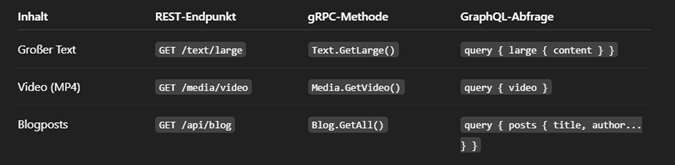
\includegraphics[width=0.7\textwidth]{images/prakt1.png}
	\caption{Daten}
\end{figure}

Die Struktur des Backend-Services gliedert sich in 4 eigenständige Projekte:

\begin{enumerate}
\item Common:
Das Common Projekt stellt die Testdaten zentral zur Verfügung. Damit die Testdaten bei einem Request nicht zuerst aus der Datei gelesen werden müssen, werden diese bei Programmstart einmal in den Arbeitsspeicher geladen. Zu diesem Zweck wurde ein API – Cache erstellt, der alle Text und Medienobjekte vorab einliest, die Daten können dann zur Laufzeit direkt vom Cache abgefragt werden.
 
Für die Testdaten wurden Datentypen die typischerweise an Web Clients gesendet werden ausgwählt und beinhalten:


\begin{itemize}
	\item Texte in drei Größen: 1\,kB, 10\,kB, 100\,kB
	\item Medieninhalte: 3\,MB Foto, 30\,MB Audio-Datei, 100\,MB Video-Datei
	\item Strukturierte Binärdaten: ein selbst definierter Datentyp mit verschachtelten Abschnitten, Metadaten, Zahlenblöcken und Autoreninformationen
\end{itemize}
\item RestAPI:
Die REST API wurde mittels einem Controller Muster von ASP.NET Core implementiert und stellt 3 eigenständige Endpunkte zur Verfügung. Die Kommunikation erfolgt ausschließlich über http GET.

Die Controller sind wie folgt definiert:

\begin{itemize}
	\item \textbf{TextController}: Stellt Textdaten in drei Größen zur Verfügung.\\
	\emph{Rückgabeformat}: \texttt{application/json}
	\item \textbf{MediaController}: Stellt ein Bild, eine Audiodatei und ein Video bereit.\\
	\emph{Rückgabeformat}: Binärdaten (\texttt{byte[]}) mit MIME-Type \texttt{image/jpeg}, \texttt{audio/wav}, \texttt{video/mp4}
	\item \textbf{BlogController}: Stellt einen vordefinierten Blogeintrag bereit.\\
	\emph{Rückgabeformat}: \texttt{application/json}
\end{itemize}

\item GraphQlAPI:
Die GraphQL-API wurde mittels des \texttt{.NET}-Frameworks \texttt{HotChocolate} implementiert.
Als Einstiegspunkt wurde eine \texttt{Query}-Klasse definiert, welche für die verschiedenen Services (Text, Medien, Blog) mit jeweiligen Teildateien erweitert wurde.

Folgende Queries wurden definiert:
\begin{itemize}
	\item \textbf{TextQuery}: Stellt die Felder \texttt{small}, \texttt{medium} und \texttt{large} bereit, welche jeweils Textinhalte als \texttt{string} zurückgeben.
	\item \textbf{MediaQuery}: Stellt die Felder \texttt{image}, \texttt{audio} und \texttt{video} bereit, welche in der GraphQL-Antwort Base64-kodiert übertragen werden.
	\item \textbf{BlogQuery}: Stellt das Feld \texttt{posts} zur Verfügung, welches die für den Blogpost definierten Daten enthält.
\end{itemize}

Alle Abfragen erfolgen über \texttt{HTTP~POST}-Anfragen an den Endpunkt \texttt{/graphql} und haben das Format \texttt{application/json}.

\item GrpcWebAPI: 
Die gRPC-Web-API basiert auf den definierten \texttt{.proto}-Dateien (\texttt{text.proto}, \texttt{media.proto}, \texttt{blog.proto}). In den Proto-Dateien wurden sowohl die \emph{Messages} und Datentypen der Testdaten als auch die \emph{Services}, mit denen auf die Messages zugegriffen werden kann, definiert. 

Die Services implementieren folgende Methoden:
\begin{itemize}
	\item \textbf{TextService}: Rückgabe der drei Textgrößen über die Methoden \texttt{GetSmall()}, \texttt{GetMedium()} und \texttt{GetLarge()}.\\
	\emph{Rückgabeformat}: \texttt{TextResponse}-Message mit einem \texttt{string}-Feld (\texttt{content}), serialisiert im Protocol-Buffers-(binary)-Format.
	
	\item \textbf{MediaService}: Streaming von Binärdaten in 64\,kB-Chunks über die Methoden \texttt{GetImage()}, \texttt{GetAudio()} und \texttt{GetVideo()}. Anders als bei den anderen Services werden hier die Mediendateien nicht als vollständige Datei, sondern als 64\,kB-Chunks gestreamt. Da gRPC nicht dafür konzipiert wurde, große Dateien am Stück zu übertragen, ist dies die empfohlene Vorgehensweise für den Umgang mit großen Dateien. Bei REST und GraphQL hingegen wurde auf ein solches Streaming verzichtet, da entsprechende Mechanismen nicht nativ unterstützt werden.\\
	\emph{Rückgabeformat}: Server-Streaming von Chunk-Nachrichten (\texttt{bytes}-Feld), serialisiert als Protocol-Buffers-Stream über HTTP/2.
	
	\item \textbf{BlogService}: Rückgabe strukturierter Blogposts via \texttt{GetAll()}.\\
	\emph{Rückgabeformat}: \texttt{BlogPostsResponse} (Liste von \texttt{BlogPost}-Nachrichten), ebenfalls als Protocol Buffers (binary) kodiert.
\end{itemize}

Die API wurde so konfiguriert, dass sowohl normales gRPC als auch gRPC-Web verwendet werden kann. Die Implementierung für gRPC-Web wird mittels des Pakets \texttt{Grpc.AspNetCore.Web} bereitgestellt. Die Generierung der gRPC-eigenen Klassen erfolgte mittels \emph{gRPC Tools}. \emph{gRPC Tools} erstellt dabei bei jedem Build die im Proto-File definierten Klassen, die anschließend im Code verwendet werden können.

\begin{table}[h]
	\centering
	\caption{Verwendete Technologien}
	\begin{tabular}{lll}
		\hline
		\textbf{Komponente} & \textbf{Technologie/Tool} & \textbf{Version} \\
		\hline
		Backend-Framework & \texttt{.NET~SDK} & 9.0 \\
		REST API & \texttt{ASP.NET~Core~Web~API} & 9.0.5 \\
		GraphQL & \texttt{HotChocolate} & 15.1.5 \\
		gRPC & \texttt{Grpc.AspNetCore} & 2.71.0 \\
		gRPC-Web & \texttt{Grpc.AspNetCore.Web} & 2.71.0 \\
		Protobuf Tools & \texttt{Grpc.Tools} / \texttt{protoc} & 2.72.0 \\
		\hline
	\end{tabular}
\end{table}

\subsubsection{Web-Client:}
Um die Messungen aus der Sicht eines Front-End-Clients durchzuführen, wurde ein Web-Client erstellt, von dem aus die jeweiligen Requests gesendet werden können und der die gemessenen Daten grafisch darstellt. Neben der grafischen Darstellung werden im Client auch die End-to-End-Latenz und die Payloadgröße ermittelt. Die Anwendung wurde mit \texttt{React} und \texttt{TypeScript} erstellt und mithilfe von \texttt{Vite} gebündelt und lokal bereitgestellt.

\subsection*{Architektur und Aufbau}
Der Web-Client dient primär als Simulation eines realen Benutzerverhaltens einer Front-End-Anwendung. Über ein einfaches Interface kann ausgewählt werden:
\begin{itemize}
	\item Gegen welche API-Schnittstelle (\texttt{REST}, \texttt{GraphQL}, \texttt{gRPC-Web}) ein Request ausgeführt werden soll
	\item Welche Datenart (Text, Medien, strukturierter Blog-Inhalt) und welche Datenmenge übertragen werden soll
	\item Ob ein einzelner Request oder eine Mehrfachanfrage parallel durchgeführt werden soll
\end{itemize}

Sowohl bei REST als auch bei GraphQL wird im Frontend die browsernative \texttt{fetch}-API für die Kommunikation mit dem Backend verwendet.  
Für die Kommunikation mit der gRPC-Web-Schnittstelle werden gRPC-Bibliotheken eingesetzt. Die Generierung der gRPC-Klassen erfolgt mittels der \texttt{ts-protoc-gen}-Bibliothek mit folgendem Befehl:

\begin{verbatim}
	npx protoc --ts_out src/api/generated --proto_path=src/proto src/proto/*.proto
\end{verbatim}

\subsection*{Clientseitige Datenverarbeitung}
Nach erfolgreichem Empfang der Daten vom Server müssen die Daten vom Client verarbeitet werden, damit diese anschließend verwendet werden können. Abhängig vom ausgewählten API-Typ und der Datenmenge werden die Daten jeweils unterschiedlich verarbeitet. 

\paragraph{Textdaten}
\begin{itemize}
	\item Bei REST und GraphQL erfolgt das Parsen des gesendeten JSON mittels der nativen \texttt{fetch}-API.
	\item Bei gRPC-Web wird die Protobuf-Nachricht automatisch über die generierten TypeScript-Klassen des \texttt{protobuf-ts}-Plugins deserialisiert.
\end{itemize}

\paragraph{Mediendaten}
Medieninhalte werden binär als \texttt{byte[]} übertragen.
\begin{itemize}
	\item Bei REST erfolgt der Empfang direkt als Blob über \texttt{response.blob()}.
	\item Bei GraphQL werden die Binärdaten Base64-kodiert als String im JSON-Response übertragen und im Client manuell dekodiert.
	\item Bei gRPC-Web werden die Binärdaten als Daten-Chunks gestreamt. Die Chunks werden im Client rekonstruiert.
\end{itemize}

\paragraph{Blogdaten}
\begin{itemize}
	\item Bei REST und GraphQL werden JSON-Objekte mit verschachtelter Struktur geparst.
	\item Bei gRPC-Web erfolgt die Deserialisierung über generierte Protobuf-Klassen.
\end{itemize}

\begin{table}[h]
	\centering
	\caption{Verwendete Frontend-Technologien}
	\begin{tabular}{lll}
		\hline
		\textbf{Komponente} & \textbf{Technologie/Tool} & \textbf{Version} \\
		\hline
		Frontend-Framework & \texttt{React} & 19.1.0 \\
		Bundler & \texttt{Vite} & 6.3.5 \\
		TypeScript Compiler & \texttt{TypeScript} & 5.8.3 \\
		REST & \texttt{fetch API} (Browser native) & (native) \\
		GraphQL Client & \texttt{fetch API} (Browser native) & (native) \\
		gRPC-Web Transport & \texttt{grpcweb-transport} & 2.11.0 \\
		Protobuf TS Plugin & \texttt{protobuf-ts} & 2.11.0 \\
		Protoc Codegen Plugin & \texttt{ts-protoc-gen} & 0.15.0 \\
		gRPC-Web Codegen & \texttt{protoc-gen-grpc-web} & 1.5.0 \\
		\hline
	\end{tabular}
\end{table}

\subsubsection{Konsolen-Client}
Die Messung des Konsolen-Clients erlaubt auch die Implementierung von gRPC. Dadurch können Response-Zeiten zwischen gRPC und gRPC-Web direkt miteinander verglichen werden. Außerdem kann aufgezeigt werden, wie sich gRPC-Technologien, welche für Microservice-Architekturen erstellt wurden, im direkten Vergleich zur Kommunikation zu Web-Clients verhalten. 

Der Konsolen-Client kann alle unterstützten APIs (\texttt{REST}, \texttt{GraphQL}, \texttt{gRPC} und \texttt{gRPC-Web}) ansprechen und führt Messungen über ein textbasiertes Menüsystem durch.  
Es werden nur Einzel-Requests unterstützt.

\subsection*{Kommunikationsmechanismen}
Die Kommunikation erfolgt jeweils über folgende Mechanismen:
\begin{itemize}
	\item \textbf{REST}: per \texttt{HttpClient} mit JSON-Deserialisierung
	\item \textbf{GraphQL}: per \texttt{GraphQL.Client}-Bibliothek
	\item \textbf{gRPC}: über \texttt{Grpc.Net.Client} direkt als native gRPC-Kommunikation
	\item \textbf{gRPC-Web}: über \texttt{Grpc.Net.Client.Web} mittels spezieller Web-Handler, angepasst an das gRPC-Web-Protokoll
\end{itemize}

Die interne Verarbeitung wurde so implementiert, dass die Messungen der Response-Zeit analog zum Web-Client das Empfangen und anschließend das Parsen beinhalten.  
Bei den Mediendaten findet auf Client-Seite keine weitere Verarbeitung des \texttt{byte[]}-Arrays statt, daher ist hier eine Gegenüberstellung zum Web-Client nicht sinnvoll.

\begin{table}[h]
	\centering
	\caption{Verwendete Technologien des Konsolen-Clients}
	\begin{tabular}{lll}
		\hline
		\textbf{Komponente} & \textbf{Technologie/Tool} & \textbf{Version} \\
		\hline
		Client-Framework & \texttt{.NET~SDK} & 9.0 \\
		GraphQL Client & \texttt{GraphQL.Client} & 6.1.0 \\
		GraphQL Client Serializer & \texttt{GraphQL.Client.Serializer.Newtonsoft} & 6.1.0 \\
		gRPC Client & \texttt{Grpc.Net.Client} & 2.71.0 \\
		gRPC-Web Client & \texttt{Grpc.Net.Client.Web} & 2.71.0 \\
		gRPC Code Generator & \texttt{Grpc.Tools} & 2.72.0 \\
		\hline
	\end{tabular}
\end{table}
	
\end{enumerate}

\clearpage
\subsection{Spezifikationen des Testsystems}
Um die Messergebnisse korrekt und vergleichbar einordnen zu können, ist es notwendig darzustellen, unter welchen technischen Rahmenbedingungen die jeweiligen Messungen durchgeführt wurden. Da die Leistungsfähigkeit der Hardware sowie die Softwareversionen die Messzeiten beeinflussen können, werden in diesem Abschnitt die relevanten Komponenten des Testsystems dargestellt.

Für die Messungen wurde folgendes Testgerät verwendet:  
Lenovo ThinkPad X1 Carbon der 10.\ Generation (Modellbezeichnung: 21CB)

\paragraph{Hardwarekonfiguration}
\begin{itemize}
	\item \textbf{Prozessor (CPU)}: 12th Gen Intel\textsuperscript{\textregistered} Core\texttrademark{} i5-1245U, 1600\,MHz, 10~Kerne
	\item \textbf{Arbeitsspeicher (RAM)}: 16\,GB LPDDR5, 5200\,MT/s
	\item \textbf{Massenspeicher (SSD)}: 512\,GB NVMe SSD
\end{itemize}

\paragraph{Betriebssystem}
Microsoft Windows 11 Pro (Version: 10.0.26100, Build 26100)

\clearpage
\subsection{Messung}
Ziel der Messungen ist es, die End-to-End-Latenz und Performance bei der Datenübertragung zwischen Front-End und Back-End zu quantifizieren und somit die im theoretischen Teil beschriebenen Eigenschaften der verschiedenen API-Technologien zu vergleichen.  
Die Responsezeiten beschreiben die tatsächliche Zeit, bis die jeweiligen Daten im Client bereitstehen (Datenübertragung und Parsing). Dabei wurden unterschiedliche Datenarten verwendet, die häufig in der Frontend-zu-Backend-Kommunikation zum Einsatz kommen.  

Untersucht wurde die Response-Zeit von Einzel-Requests, Mehrfachabfragen (20 parallele Requests) und browserabhängige Unterschiede in einem Web-Client. Zusätzlich wurden alle Technologien, einschließlich gRPC, im Konsolen-Client getestet, um Unterschiede zwischen browserbasierter und microservice-orientierter Kommunikation sichtbar zu machen und Unterschiede zwischen gRPC und gRPC-Web zu ermitteln.

Die Ergebnisse der Messungen liefern eine Grundlage zur Beantwortung der Forschungsfragen, inwiefern sich die Schnittstellentechnologien hinsichtlich der Effizienz und Eignung für typische Frontend-Szenarien unterscheiden.  
Die nachfolgenden Abschnitte stellen die gemessenen Daten dar und geben einen direkten Vergleich der Technologien.

\clearpage
\subsubsection*{Messdaten: Web-Client (Einzel-Request)}

Bei der Messung der End-To-End Latenz ergaben sich zwischen den einzelnen Technologien erhebliche Unterschiede. 
Für eine sinnvolle Auswertung der Daten, wurden jeweils 30 Requests unabhängig voneinander durchgeführt die Durschnittszeiten und der Median der aus den gemessenen Daten ermittelt. 


\textbf{TextService:}  
Es ist zu erkennen, dass kleinere Textdaten (1kB – 10 kB) von allen Schnittstellen relativ schnell verarbeitet werden konnten. gRPC Web und GraphQL weisen hierbei jedoch die geringsten Antwortzeiten auf ( 7-8 ms ), REST benötigte ca 8-9 ms für kleinere Textdaten. Bei größeren Textmengen von ( 200 kB ) steigt die Latenz erwartungsgemäß bei allen Technologien etwas an, wobei diese bei GraphQl mit 10 ms und REST mit 13 ms deutlich schneller als bei gRPC Web ( 19 ms ) bereitstehen. 

\textbf{MediaService:}  
Besonders Auffällig ist der Leistungsunterschied bei der Übertragung von Mediendaten.
Hierbei war entgegen der theortischen Erwartungen REST die schnellste Technologie für alle Medienarten. Für Bilder ( 4MB) lag dabei die mittlere Antwortzeit bei 36 ms, deutlich vor gRPC ( 182 ms ) und GraqhQL ( 511 ms ).
Ähnliches Verhalten zeigte sich bei der Übertragung von Audiodateien (30 MB), hierbei wurde mit REST eine mittlere Antwortzeit von 150 ms gemessen, mit deutlichem Abstand gefolgt von gRPC ( 2372 mms) und GraphQL ( 5870  ms ).
Bei der Übertagung von Videodaten (100 MB ) konnte in Chrome keine vergleichbare Messung der Antwortzeiten durchgeführt werden. Die Übertragung war nur über die REST-API erfolgreich. Es ergab sich dabei eine durchschnittliche Antwortzeit von 365 ms. Wegen großer Ladezeit bzw. Instabilitäten des Clients konnten für graphQL und Grpc-WEB keine Daten gemessen werden. 


\textbf{BlogService:}  
Bei der Messung der Blog-Datenstrukturen, konnten geringe Unterschiede in den Abfragezeiten zwischen den Technologien identifiziert werden. GraphQl war hierbei mit einer mittleren latenz von 7.6 ms leicht schneller als gprc ( 7.9 ms / 7.8 ms) und Rest ( 8.6 ms.

\clearpage
\subsubsection{Browser-Vergleich}
Derselbe Versuch mit Einzel-Requests wurde anschließend in zwei weiteren Web Browsern durchgeführt, um festzustellen, ob es bei der Performance der APIs eine Abhängigkeit vom Webbrowser gibt. 
Bei der Messung wurden jeweils 10 Requests pro Technologie und Service durchgeführt und daraus der Durchschnitt und der Median ermittelt.


\textbf{Textdaten:}  
Bei den Messungen reagierte Edge in allen Schnittstellen mit den niedrigsten Antwortzeiten. Vorallem bei REST und GraphQL konnten deutliche Unterschiede gemessen werden, hierbei hatte REST in Edge für kleine Textdaten im Mittel nur etwa 4-6 ms, während Chrome und Firefox 8-9 ms benötigten. Bei größeren Textmengen blieg Edge mit 9.5 ms bei Rest im Vergleich zu 13 ms in Chrome und 11 ms in Firefox weiterhin am besten.
Auch gRPC konnte in Edge am schnellsten verarbeitet werden, wobei bei größere Textdaten sowohl Edge und Chrome 19 ms benötigen und Firefox 24 ms. 


\textbf{Medieninhalte (Foto, Audio, Video)}  
Beim Senden von Mediendaten hatte hatten Chrome und Edge im Gegensatz zu Edge eine ähnlich gute Performance. Bei REST und gRPC konnte Edge und Chrome die kürzesten Antwortzeiten für Fotos ( 36 ms) und Audiodateien ( 150 ms)  liefern. Bei Firefox lagen diese bei REST bei 55 ms und 250 ms bzw. bei gRP-Web bei 250 ms und 2455 ms.

Bei dem Senden von Videodaten war Chrome am performantesten. Hier hatte REST eine Antwortzeit von 365 ms, Edge 423 ms und Firefox 676 ms. Im Gegensatz zu Chrome, konnten das Video in Firefox mit gRPC (8984 ms) und Edge ( 7984) und in Firefox auch mit GraphQL (90091 ms), auch wenn sehr langsam, dargestellt werden.


\textbf{Blogdaten:}  
Ähnliche Ergebnisse wie bei Textdaten: Edge meist am schnellsten, gefolgt von Chrome, dann Firefox.

\clearpage
\subsubsection{20 parallele Requests}
Bei der Durchführung von 20 parallelen Requests wurden jeweils pro API und Service 30 Messwerte ( bei MedienService Messwerte) gemessen und anschließend der Durchschnittswert und Median berechnet. Es zeigten sich erwartungsgemäß höhere Latenzen gegenüber denr Einzelabfragen. 

\textbf{TextService:}  
Während kleinere Textdaten noch performant verarbeitet werden können, nehmen die Unterschiede bei größeren Lasten stärker zu. Bei sehr kleinen Textdaten von 1 KB sind gRPC und graphql jeweils mit ungefähr 30 ms gleich auf, bei 10 kB ist graphQl mit 35 ms ungefähr 9 ms schneller als gRPC mit 44 ms. je größer die Daten werden, desto langsamer wird gRPC. Rest benötigte dabei jeweils 45 ms btw. 62 ms. Auch bei größeren Textdaten ist graphQl mit je 71 ms am schnellsten, gefolgt von REST mit 92 ms und gRPC mit 145 ms. 

\textbf{MediaService:}  
Bei der Verarbeitung von Medien kam es wie bereits durch die einzelabfragen erwartet zu größeren unterschieden. REST schnitt auch hier mit 384 ms für Fotos, 2420 ms für Audiodaten am besten ab. Gefolgt von gRPC mit 5736 ms für das Foto und 126026 ms für die Audiodatei. Bei GraphQl dauerte der Request für die Fotodaten 16159 ms.
Für Videodateien bzw. Audiodateien ( GraphQl ) wurde in dieser Testreihe aufgrund der bereits in den Einzelabfragen instabilen Ladeverhaltens, keine weiteren Messungen vorgenommen.


\textbf{BlogService:}  
Bei den Abfragen der Blogdaten lagen die Antwortzeiten aller Technologien im zweistelligen ms bereich. Ähnlich wie bei geringen Textdaten, sind gRPC und graphQl mit jeweis 34 ms gleichauf, gefolgt von REST mit 53 ms.

\clearpage
\subsubsection{Messungen im Konsolen-Client}
Um die Kommunikationsleistung der einzelnen Technologien ohne Einfluss eines Browers zu ermitteln, und um einen direkten Performancevergleich zwischen gRPC und gRPC-Web zu ermitteln wurden ebenfalls Messungen in der Kommunikation innerhalb einer Microservice basierten Architektur untersucht. Wie erwartet sind die Messewerte in dieser Messung zum größten Teil deutlich besser als zwischen Web-Client und Backend Service.  

\textbf{TextService:}  
Alle viel Technologien zeigten bei kleinen und mittleren Textdaten sehr geringe Antwortzeiten. gRPC hatte hier jedoch die schnellste respond Zeit mit nur ungefähr 1 ms. REST, GraphQl und gRPC haben ungefähr die selbe Zeit von 2-3 ms.
Auch bei großen Textdaten ist gRPC mit 4.1ms am schnellste, gefolgt von GraphQl mit 5.5 ms, REST mit 6.4 ms und gRPC Web mit 6.8 ms.


\textbf{MediaService:}  
Bis auf REST, war die Übertragung der Mediadaten im Konsolen-Client schneller als im Web-Client. gRPC hatte mit 43 ms die schnellste Übertragung von Fotos gefolgt von REST mit 46 ms, gRPC Web mit 51 ms und GraphQL mit 5716 ms. Bei den 30 Mb Audiodaten sind REST, gRPC und gRPC-Web gleichauf mit 250 ms. Nur bei großen Binärdaten ist REST mit 540 ms schneller als gRPC (610) und gRPC-Web (705 ms). Für GraphQL konnte keine sinnvolle Messung für Audio oder Fotos durchgeführt werden.

\textbf{BlogService:}  
Bei den Senden von strukturierten Bloddaten liegen gRPC und REST mit ungefähr 1 ms ungefähr gleich auf, gefolgt von GraphQl mit 2,4 und gRPC-Web mit 2.9 ms.

\clearpage
\subsubsection*{Fazit der Messungen}
Aus den mit den Prototypen durchgeführten Messungen, können einige Annahmen getroffen und Unterschiede aufzeigen. Zu einem großen Teil konnten die im theoretischen Teil beschriebenen Annahmen zu den Unterschieden zwischen REST, GraphQl, gRPC und gRPC-Web bestätigt werden, gleichzeitig wurden einige andere Erkenntnisse hervorgebracht. Folgende Unterschiede bzw. Erkenntnisse konnten gewonnen werden:

\chapterend


\end{document}